%%%%%%%%%%%%%%%%%%%%%%%%%%%%%%%%%%%%%%%%%%%%%%%%%%%%%%%%%%%%%%%%%%%%%
% LaTeX Template: Project Titlepage Modified (v 0.1) by rcx
%
% Original Source: http://www.howtotex.com
% Date: February 2014
% 
% This is a title page template which be used for articles & reports.
% 
% This is the modified version of the original Latex template from
% aforementioned website.
% 
%%%%%%%%%%%%%%%%%%%%%%%%%%%%%%%%%%%%%%%%%%%%%%%%%%%%%%%%%%%%%%%%%%%%%%

\documentclass[11pt]{report}
\usepackage[a4paper]{geometry}
\usepackage[myheadings]{fullpage}
\usepackage{fancyhdr}
\usepackage{lastpage}
\usepackage{graphicx, wrapfig, subcaption, setspace, booktabs}
\usepackage[T1]{fontenc}
\usepackage[font=small, labelfont=bf]{caption}
\usepackage{fourier}
\usepackage[protrusion=true, expansion=true]{microtype}
\usepackage[english]{babel}
\usepackage{sectsty}
\usepackage{url, lipsum}
\usepackage{amsmath}

\newcommand{\HRule}[1]{\rule{\linewidth}{#1}}
\onehalfspacing
\setcounter{tocdepth}{5}
\setcounter{secnumdepth}{5}

%-------------------------------------------------------------------------------
% HEADER & FOOTER
%-------------------------------------------------------------------------------
\pagestyle{fancy}
\fancyhf{}
\setlength\headheight{15pt}
\fancyhead[L]{Terrence Ho}
\fancyhead[R]{Experiment 6 $\&$ 7}
\fancyfoot[R]{Page \thepage\ of \pageref{LastPage}}
%-------------------------------------------------------------------------------
% TITLE PAGE
%-------------------------------------------------------------------------------

\begin{document}

\title{ \normalsize \textsc{Physics 4AL}
        \\ [2.0cm]
        \HRule{0.5pt} \\
        \LARGE \textbf{\uppercase{Experiment 6 $\&$ 7: Harmonic Oscillator:
        Physical Pendulum and Waves on a Vibrating String}}
        \HRule{2pt} \\ [0.5cm]
        \vspace*{2\baselineskip}}

\date{}

\author{
        Terrence Ho | ID: 804793446 \\ 
        Date of Lab: May 23th and 30th, 2017 \\
        Lab Section: Tuesday, 5 P.M.\\
        T.A.: David Bauer\\
        Lab Partners: Robathan Harries \\
        Abstract: 165 words\\
        Report: 2189 words\\
    }
\maketitle
\tableofcontents
\newpage

%-------------------------------------------------------------------------------
% Section title formatting
\sectionfont{\scshape}
%-------------------------------------------------------------------------------

%-------------------------------------------------------------------------------
% BODY
%-------------------------------------------------------------------------------
\addcontentsline{toc}{section}{Abstract}
\begin{center}
\title{
    \Large \textbf{\uppercase{Investigating Harmonic Motion of a Physical
    Pendulum and the Waves of a vibrating spring}}
}


T. Ho\footnote{Henry Samueli School of Engineering and Applied Science,
University of California, Los Angeles}
\end{center}

In mechanical physics, harmonic motion is the oscillatory motion of an object
where the restoring force increases with displacement and opposite the direction
of motion.  Harmonic motion can occur with a physical pendulum if it is
displaced from its equilibrium position.  Harmonic motion also occurs in
non-rigid objects, such as a string, where each particle of the string is
vibrated and oscillates back and forth. We sought to study these two forms of
harmonic motion in our experiment.  Specifically we studied frequencies of
damped and driven oscillations for physical pendulums, to gain an understanding
of how oscillations are controlled and created.  We found the resonant frequency
was 0.714 $\pm$ 0.005 Hz.  In the second part of our experiment, we measured the
wave speed travelling along a vibrating spring, and investigated the effects of
adding a boundary condition to the middle of the string. The wave speed
calculated in our experiment was $\pm$ m/s.

\newpage

\section*{Introduction}
\addcontentsline{toc}{section}{Introduction}
Sidney Colman once said: "The career of a young theoretical consists of treating
the harmonic oscillator in ever-increasing levels of abstraction." However, even
at a level with no abstractions, we examples of harmonic oscillations in many
systems of motion; we studied two of these systems in this experiment, one involving 
a physical pendulum and the other vibrating strings. Although these two motions 
may seem physically very different, a model of harmonic motions can be found 
in both physical systems.

With the pendulum, we examined two areas of harmonic motion: damping and driven
harmonic motion. Damping occurs when an external force results in a decrease in
amplitude over time. There are three damping regimes, underdamped, overdamped, and 
critically damped. We also studied driven harmonic motion with our swinging pendulum.
The driving frequency occurs when the oscillatory motion produced by a constant
outside force is at its greatest.  

Vibrating strings are also a interesting because the vertical motion induced on
a string creates an oscillatory motion similiar to that of a physical pendulum. 
Each particle on a string oscillates in relation to particles near it.
Furthermore, if the string is vibrated at certain frequencies, the string 
produces standing waves, with the number of waves varying with the frequency 
at which the wave is vibrated at. We investigate these properties of vibrating 
strings in our experiment. (More?)

\section*{Methods}
\addcontentsline{toc}{section}{Methods}

\begin{figure}[h!]
    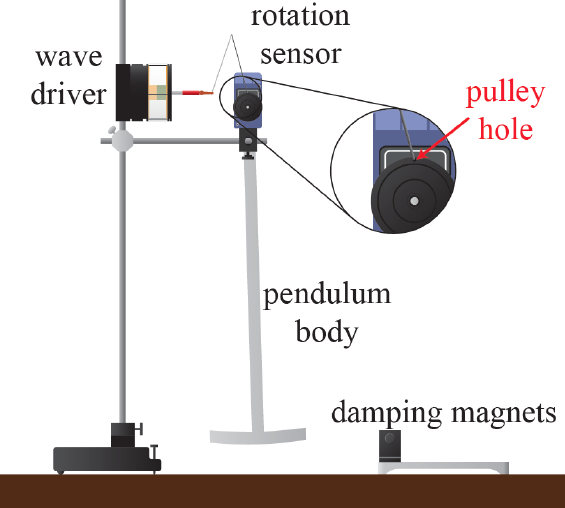
\includegraphics[width=\linewidth]{Part1Setup.png}
    \captionsetup{labelformat=empty}
    \caption{\textbf{Figure 6.1 Set up for Part I of Physical Pendulum}  Figure
    reproduced (with permission) from Fig 6.1 by Campbell, W. C. et al.$^1$}
\end{figure}

\subsection*{Part I}
\addcontentsline{toc}{subsection}{Part I}
In the first part of our experiment, we setup our equipment in the fashion shown
in \textbf{Figure 6.1}.  (We used a photogate to determine a start position
from which to release the pendulum from.)  We attached a wave driver and rotation
sensor to our recording equipment, and set a high sampling rate to record data at, 
perhaps 50 Hz (If it is too low, the maxima in wave patterns can't be detected).
We did six trials with the pendulum, one without the damping magnets and 5 with.
For each trial, we recorded the time and angle of the pendulum as it oscillated.
We also wanted to dertemine critical damping, so we looked at our five previous
damped trials to approximate where the critical damping spot was and adjusted the 
magnet spacing until we achieved critical damping

Next, we began the harmonic motion with driving part of the experiment. We set the
magnet spacing so that the magnets will damp out the free undriven oscialltions
in about 5 to 10 seconds, (in our case 30 mm).  We first want to find the
damped, driven resonant frequency \(\omega_r\).  Record three Lissajous figures
whose x-axis are Output Voltage (V) and y-axis is angle(rad),
one at the resonant frequency, one below the resonant frequency, and one above. 
We determined the driven resonant frequency by looking for the Lissajous plot
that was symmetric.  

Lastly, using the drive frequency we found in the last part, we recorded frequency
and amplitudes of ten different drive frequencies. When plotted, this data should
appear similar to a resonant curve, with the drive frequency as the peak.

\begin{figure}[h!]
    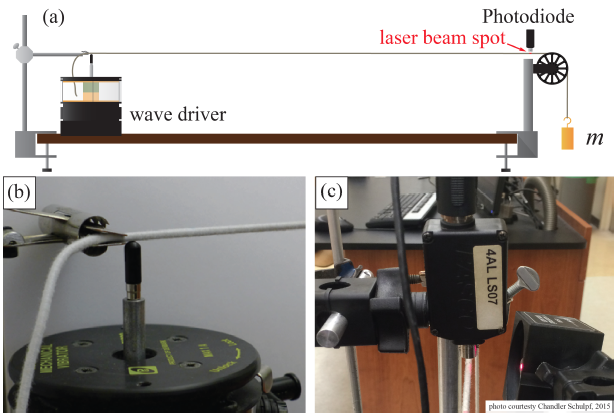
\includegraphics[width=\linewidth]{Part2Setup.png}
    \captionsetup{labelformat=empty}
    \caption{\textbf{Figure 6.2 Set up for Part II of Experiment}  Equipment
        shown above used to study waves on a vibrating string.  (a) and (b) depict a
driver that produces vibrations on the string.  The vibrations are monitored by
a photodetector that shines a laser beam onto the string in (c). Figure
reproduced (with permission) from Fig. 7.1 by Campbell, W. C. et al.$^1$}
\end{figure}

\subsection*{Part II}
\addcontentsline{toc}{subsection}{Part II}

In Part II of our experiment we studied waves of a vibrating spring.  Our
experiment setup is shown in \textbf{Figure 6.2}. We first
wanted to measure the wave speed for several values of tension by varying the
mass hung over the wheel.  However, because linear mass density changes with
different stretching, we had to recalculate linear mass density for each trial
by dividing the mass of the string by the new length.  We took three trials of
wave speed, with at least one mass greater than 350 g (which will be used in
later parts of the experiment). We configured our signal generator according to 
\textbf{Figure 6.3}.  We set a high recording frequency to ensure the data
generated included the peaks of the oscillations, and recorded data of time (s), 
Light Intensity ($\%$), and Output Voltage Ch01 (V). 

Next, we wanted to study standing waves on a vibrating string. Using the weight
greater than 350 g, we experimented with the driving frequency until we found the
fundamental mode of resonance.  We plotted Lissajous figures once again to
find the fundamental mode.  We found the other nodes of resonance up to the tenth
node by adjusting the frequency around the nth multiple of the fundamental node.

Lastly, the string was driven at resonant frequencies for n = 2, 4, and 5 twice,
once with a clamp in the middle of the string and once without.  We recorded the
amplitudes for three frequencies.

\begin{figure}[h!]
    \centering{
        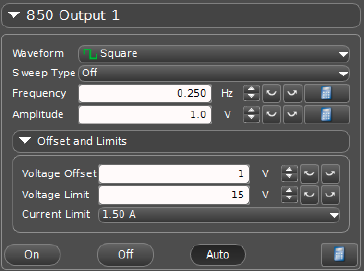
\includegraphics[]{capstoneSettings.png}
    }
    \captionsetup{labelformat=empty}
    \caption{\textbf{Figure 6.3 Caption Settings for Signal Generator}  Using
    the Signal Generator to measure wave speed.  Figure reproduced (with
permission) from Fig. 7.2 by Campbell, W. C. et al.$^1$}
\end{figure}

\section*{Analysis}
\addcontentsline{toc}{section}{Analysis}

\subsection*{Part I: Harmonic Oscillations of a Physical Pendulum}
\addcontentsline{toc}{subsection}{Part I: Harmonic Oscillations of a Physical Pendulum}

% Looking at the pendulum in \textbf{Figure 6.1},
% the torque due to gravity of a pendulum with mass \(M\), an angled height of 
% \(\theta\), with the center of mass a distance \(l\) below the pivot is given by
% \(\tau_{gravity} = -Mgl\sin(\theta)\).  The torque due to the spring at the top of the
% pendulum is given by \(\tau_{spring} = -B\sin(\theta)\cos(\theta)\).  The magnets
% at the bottom exert a damping force equal to \(\tau_{damping} =
% -b\dot{\theta}\).  The full equation of motion can be put together to get
% \(I\ddot{\theta} = -Mgl\sin(\theta) - B\sin(\theta)\cos(\theta) -
% b\dot{\theta}\).  For small angular displacements, \(\sin(\theta) \approx
% \theta\) and \(\cos(\theta) \approx 1\). Thus we can simpifly the full equation
% of motion to \(I\ddot{\theta} \approx -(Mgl + B)\theta - b\dot{\theta}\), or
% \(I\ddot{\theta} = -k\theta - b\dot{\theta}\).

% The equation of motion derived is comparable to \(m\ddot{x} = -kx - b\dot{x}\)
% (found in Experiment 5).  If we substitute \(x \rightarrow \theta\) and \(m
% \rightarrow I\) into the solution to the differential equation, we get
% \(\theta(t) = Ae^{i\sqrt{\frac{k}{I} - \frac{b^2}{4I^2}}} \times e^{-bt/2I} =
% Ae^{i\omega_{damped}t} \times e^{-bt/2I}\). Damped angular frequency is equal to 
% \(\omega_{damped} \equiv \sqrt{\frac{k}{I} - \frac{b^2}{4I^2}} = 
% \sqrt{\omega_0^2 - \frac{1}{\tau^2}}\), and damping time \(\tau \equiv
% \frac{2I}{b}\).  The undamped resonant frequency is \(\omega_o \equiv
% \sqrt{k/I}\). 

In our first part of the experiment, we looked at undriven harmonic motion of
pendulums. There are three regimes of oscillation, which were previously mentioned.
\begin{enumerate}
    \item Underdamped motion: \(\omega_0 > \frac{1}{\tau}\). 
    \item Overdamped motion: \(\omega_0 < \frac{1}{\tau}\).
    \item Critically damped motion: \(\omega_0 = \frac{1}{\tau}\).
\end{enumerate}
Damping time $\tau$ is the time it takes for an oscillation to decay exponentially by a
factor of $\frac{1}{e}$.
These three regimes of oscillatory motion are shown in \textbf{Figure 6.4}. To
obtain these figures, we recorded one trial on oscillation with no damping
magnets, then 5 trials of successively higher damping (with magnet spacing of
50 mm, 40 mm, 30 mm, 20 mm, 10mm).  Critical damping was achieved with a magnet
spacing of 15.0 $\pm$ 0.5 mm.  If the gap between magnets were less, we started
to experience overdamped motion. 

We can see that undamped motion of the pendulum in \textbf{Figure 6.4} became
experienced oscillations whose amplitudes decreased slightly over time.  On the
other hand, critically damped and overdamped oscillations reached the
equilibrium point and did not move past this point, coming to rest.  We can see
that the crticially damped oscillation reached the equilibrium point the
fastest, which is what we expect. 
We determined the \(\omega_0\) by zooming in to the underdamped graph and
looking at when the maxima of the oscillations appeared.  \(\omega_0 = 0.714
\pm 0.005\) rads/sec.


\begin{figure}
    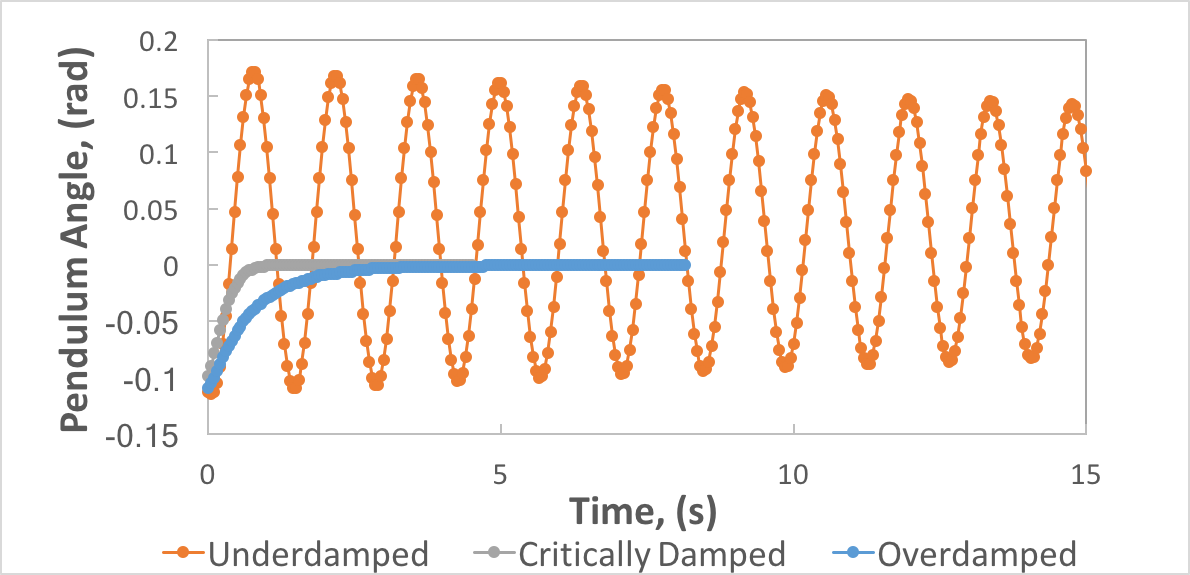
\includegraphics[width=\linewidth]{ThreeDampGraph.png}
    \captionsetup{labelformat=empty}
    \caption{\textbf{Figure 6.4 Pendulum angle against time for underdamped,
    overdamped, and critically damped motion.} The critically damped oscillation
    (with a magnet spacing of 15.0 $\pm$ 0.5 mm)
reached the equilibrium point the fastest compared to the other types of motion.
The data points were joined by lines to make sure the different types of damping
were clear.}
\end{figure}

\bigskip
In the next section of our experiment, we looked into driven oscillations.  For
the following driven damped analysis, we used a damping gap of 30 mm.
We assumed the damped driven oscillation resonance $\omega_R$ is equal to the
previously found $\omega_0$, because the damping is low.  To confirm that
\(\omega_R \approx \omega_0\), we plottedj Lissajous plots of angle and output
voltage.  We will know that we will have found $\omega_R$ when the Lissajous
plot is symmetric on both sides.  In \textbf{Figure 6.5}, we plotted three
Lissajous figures, with \textbf{(a)} being below resonance(due to left tilt), 
\textbf{(b)} being above resonance (due to right tilt), and \textbf{(c)} being 
at resonance.  

By looking at these Lissajous plots, we can determine that $\omega_R$ is indeed
0.714 $\pm$ 0.005 Hz (the uncertainty was derived by looking at the tilts of the
plots above and below resonance, and determining the difference). 

We can also determine the damping time of the physical pendulum by looking at
the peaks of \textbf{Figure 6.6} and calculating the ratios of successive
amplitudes of the peaks, using the formula \[\tau = -\frac{T}{\ln(\frac{F(t +
T)}{F(t)})}\]  We calculate that the mean damping time to be 1.86 $\pm$ 0.04 s.  

Now that we have the resonant frequency \(\omega_R\) and the damping time, we
can find th Q-factor of the physical pendulum, using the equation \[Q \equiv
\frac{1}{2}\tau\omega_R\]  We find that the Q-factor of the system is 0.66
$\pm$ 0.08 (uncertainty found by propagation of uncertainties).  


There is also another way to find the Q-factor of the system, but finding the
amplitudes of the oscillation at frequencies around the drive frequency
$\omega_R$, known as the amplitude response.  
We plotted 10 frequencies in total, some above and below the
resonant driving frequency, in \textbf{Figure 6.7}.  
We can define Q as the ratio of resonant frequency and the width of the
resonant curve, or \[Q \approx \frac{\omega_0}{\Delta\omega}\] $\Delta\omega$
is equal to $\frac{1}{\sqrt{2}}$ of the maximum amplitude, which in this case is
0.013 $\pm$ 0.009. $\Delta\omega = 0.19 \pm 0.05$.
We can find that the Q-factor = 3.76 $\pm$ 0.06 (uncertainties found by
propagation of uncertainties).

\begin{figure}
    \begin{subfigure}{.5\textwidth}
        \centering
        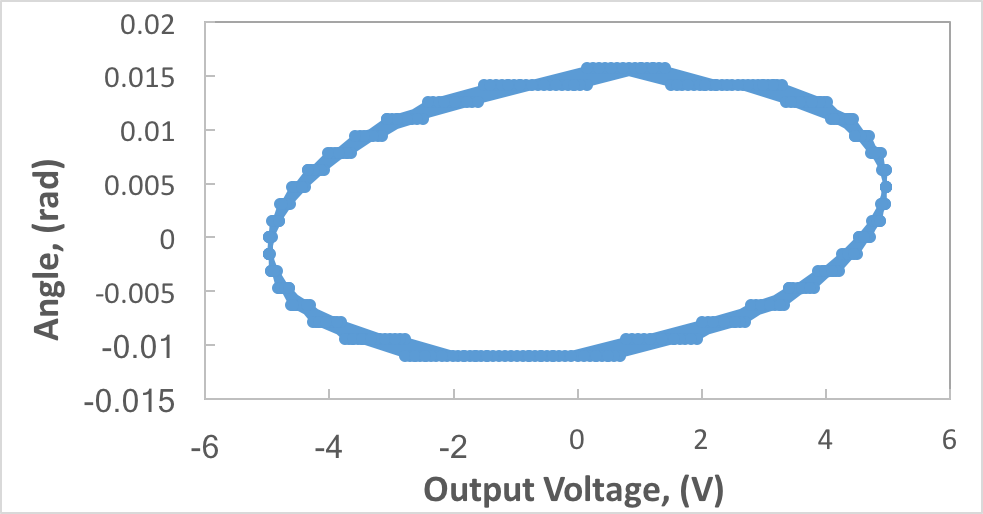
\includegraphics[width=0.95\linewidth]{LissajousLeft.png}
        \caption{}
    \end{subfigure}
    \begin{subfigure}{.5\textwidth}
        \centering
        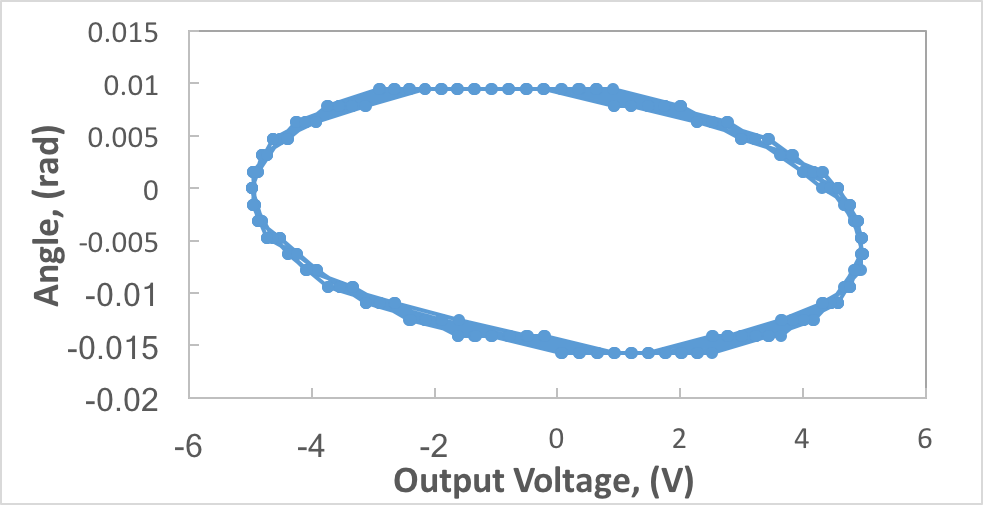
\includegraphics[width=0.95\linewidth]{LissajousRight.png}
        \caption{}
    \end{subfigure}
    \begin{subfigure}{\textwidth}
        \centering
        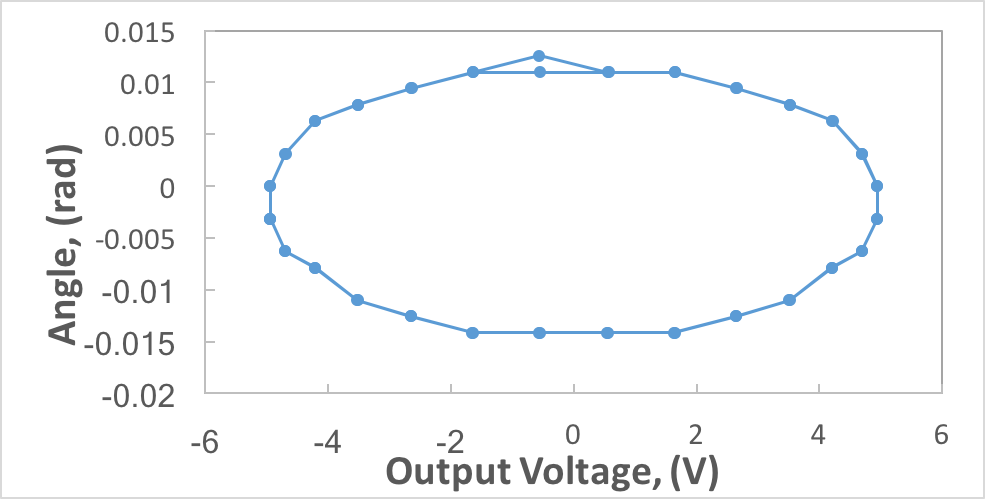
\includegraphics[width=\linewidth]{LissajousCenter.png}
        \caption{}
    \end{subfigure}
    \captionsetup{labelformat=empty}
    \caption{\textbf{Figure 6.5 Lissajous plots below, above, and at resonance.}
        Parametric plots of Angle (rad) vs Output voltage (V). (a) shows drive
    frequency below resonance, (b) shows drive frequency above resonance, and (c)
shows drive frequency at resonance. The data points are joined to make the
Lissajous Figures more apparent.}
\end{figure}

The two values of Q that are completely outside their
uncertainty boundaries. This can be caused by the large uncertainty in
finding the $\Delta\omega$. Also, the amplitude response method of
finding the Q-factor is very sensitive to exact frequencies since the amplitude is
a function of frequency. If frequency values have a large uncertainty,
then the Q-factor could end up with a large uncertainty and wrong value.


\begin{figure}
    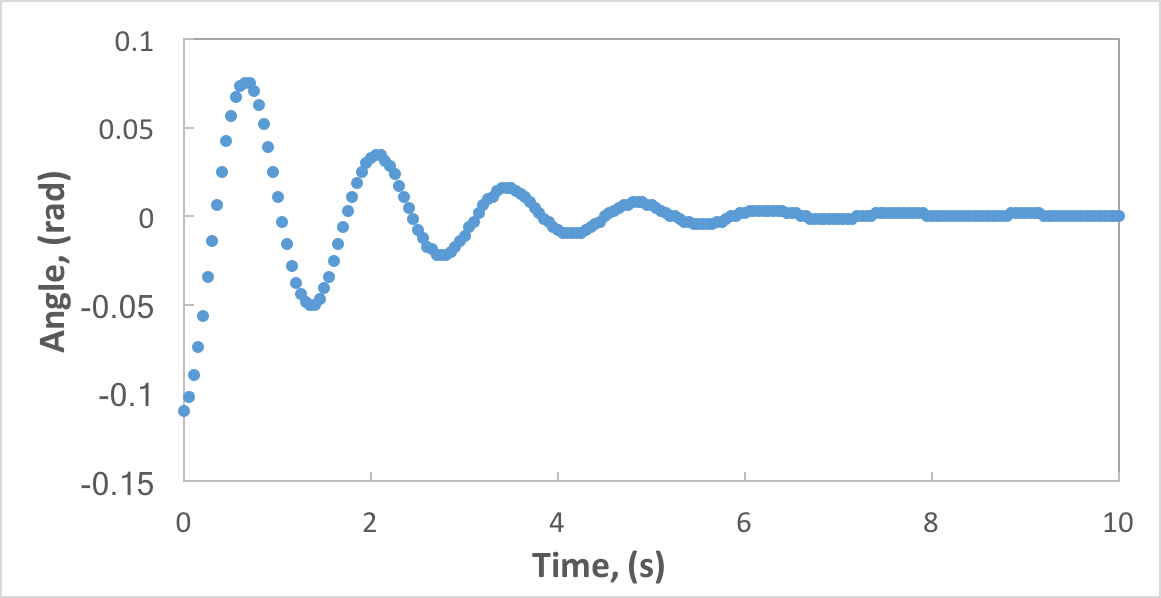
\includegraphics[width=\linewidth]{LowDamping.png}
    \captionsetup{labelformat=empty}
    \caption{\textbf{Figure 6.6 Undriven Damped Oscillations of Pendulum} The
    damping space used for this oscillation was 30 mm.}
\end{figure}

\begin{figure}
    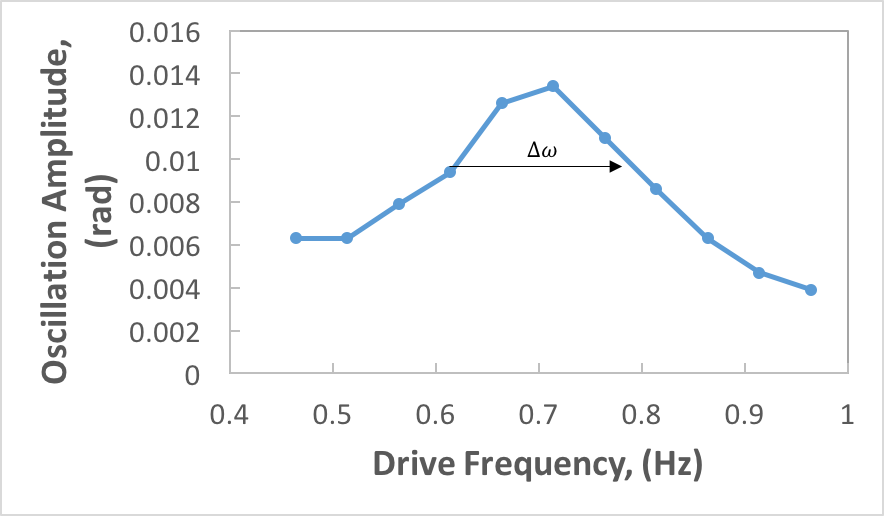
\includegraphics[width=\linewidth]{DriveFrequencyAmplitude.png}
    \captionsetup{labelformat=empty}
    \caption{\textbf{Figure 6.7 Amplitude Response of Oscillations around Drive
    Frequency} The points indicate the oscillation amplitude in radians for the
driving frequency.  By joining the points, we form a Lorentzian shape. The
resonance width is 1.9 $\pm$ 0.5 Hz.}
\end{figure}
% The equation of motion for driven oscillations looks similiar to the previous
% equation of motion, except with an added term: \(I\ddot{\theta} = -k\theta -
% b\dot{\theta} + C\cos(\omega_dt)\).  

% In a damped but driven oscillation of motion, the frequency at which the
% amplitude is at its maximum is called the driving frequency or driven resonant
% frequency \(\omega_R\).  \(omega_R\) can be obtained by solving the equation for
% driven motion and \(\omega_R = \sqrt{\omega_0^2 - \frac{2}{\tau^2}}\). 

% The driven resonance frequency can also be found by plotting Lissajous figures,
% and finding the graph whose circle is nearly symmetric. \textbf{Figure 6.5}
% shows three such figures.  \textbf{Figure 6.5 (c)} shows the driving resonant
% frequency at 0.714 $\pm$ 0.005 Hz.

% Damping time $\tau$ can be found by measuring ratios of maxima in the 
% undamped, undriven oscillations, with the equation \(\tau = -\frac{T}{ln\big(\frac{F(t +
% T)}{F(t)}\big)}\). The mean damping time was found to be 1.82 $\pm$ 0.06 s.

% The Q-factor of the system defines how ---.  We define the Q-factor to be \(Q
% \equiv \frac{1}{2}\tau\omega_R\).  Using the values of $\tau$ and $\omega_R$
% found previously, we find that Q = 0.643 $\pm$ 0.004.



\subsection*{Part II: Oscillations of a Vibrating String}
\addcontentsline{toc}{subsection}{Part II: Oscillations of a Vibrating String}

As stated before, the individual particles of a vibrating string mimic harmonic
motion by oscillating up and down.  This oscillations forms waves that travel
along the string. In the first part of our experiment we tried to predict the 
velocities of these waves as they travel along the string. 

For a string that has tension \(T\) and linear mass density \(\mu\), the wave
velocity is given by \(v = \sqrt{\frac{T}{\mu}}\).  However, because $\mu$
changes as it is stretched as a function of the length, we need to recalculate 
$\mu$ for different amounts of stretching.  

The orignal mass of the string was 0.0135 $\pm$ 0.0005 kg.  The total
unstretched length of the string used for the experiment was 1.955 $\pm$ 0.0005 m.
\textbf{Table 6.1} shows the data recorded for three different masses hung from
the string.

\begin{center}
    \begin{tabular}{| c | c | c | c | c |}
        \hline
        Mass (kg) & String Length (m) & Tension (N) & Linear Mass Density
        $\mu$ (kg/m) & Wave Velocity (m/s) \\
        \hline
        0.202 $\pm$ 0.0005 & 1.979 $\pm$ 0.0005 & 1.983 $\pm$ 0.005 & 0.0069
        $\pm$ 0.0002 & 17.0 $\pm$ 0.5 \\ 
        \hline
        0.303 $\pm$ 0.0005 & 2.002 $\pm$ 0.0005 & 2.965 $\pm$ 0.005 & 0.0068
        $\pm$ 0.0002 & 20.88 $\pm$ 0.07 \\
        \hline
        0.403 $\pm$ 0.0005 & 2.034 $\pm$ 0.0005 & 3.946 $\pm$ 0.005 & 0.0067
        $\pm$ 0.0002 & 24.3 $\pm$ 0.2 \\
        \hline
    \end{tabular}
\end{center}
\captionof*{table}{\textbf{Table 6.1} Measurements recorded to find $\mu$ and
wave velocity of the standing wave.}

\setlength{\parindent}{5ex}
As more mass is hung from the pulley and more tension is applied to the string,
the linear mass density decreases and the velocity increases. 

Wave velocity can also be calculated by graphing the Light Intensity ($\%$) and
time (s) \textbf{Figure 6.7}.  The wave velocity is calculated by dividing twice the
length of the string between the pulley and clamp (distance a wave travels) and 
dividing it by the difference in time peaks. The distance a wave travels is 3.18
$\pm$ 0.005 m.  


\begin{center}
    \begin{tabular}{| c | c | c | c |}
        \hline
        Mass (kg) & Time Interval (s)& Wave Velocity (m/s) \\
        \hline
        0.202 $\pm$ 0.0005 & 0.187 $\pm$ 0.005 & 17.0 $\pm$ 0.5\\ 
        \hline
        0.303 $\pm$ 0.0005 & 0.153 $\pm$ 0.005 & 20.8 $\pm$ 0.7\\
        \hline
        0.403 $\pm$ 0.0005 & 0.132 $\pm$ 0.005 & 24.1 $\pm$ 0.9 \\
        \hline
    \end{tabular}
\end{center}
\captionof*{table}{\textbf{Table 6.2} Wave velocities measured by photodiode
using time intervals of \textbf{Figure 6.8 (a), (b), (c)}.}

\setlength{\parindent}{5ex}
The velocities calculated in \textbf{Table 6.1} and \textbf{Table 6.2} show that
the velocities calculated from tension and $\mu$ and measured by the photodiode 
were within the same uncertainty range, and so our measured wave velocities are
precise.  

For the remaining parts of the experiment, the 0.4 kg weight was used to provide
tension. 

\begin{figure}
    \begin{subfigure}{\textwidth}
        \centering
        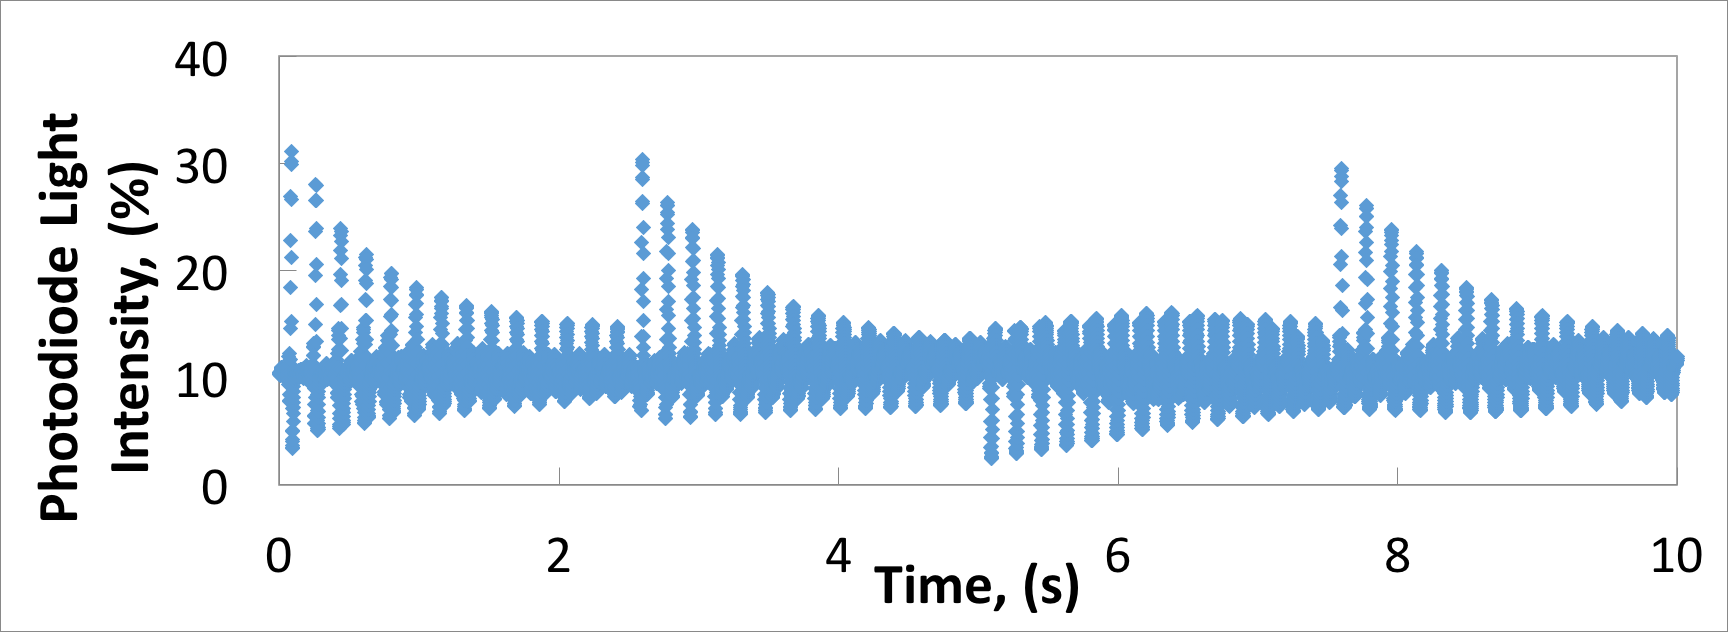
\includegraphics[width=0.95\linewidth]{LightIntensity1.png}
        \caption{Weight: 0.2 kg}
    \end{subfigure}
    \begin{subfigure}{\textwidth}
        \centering
        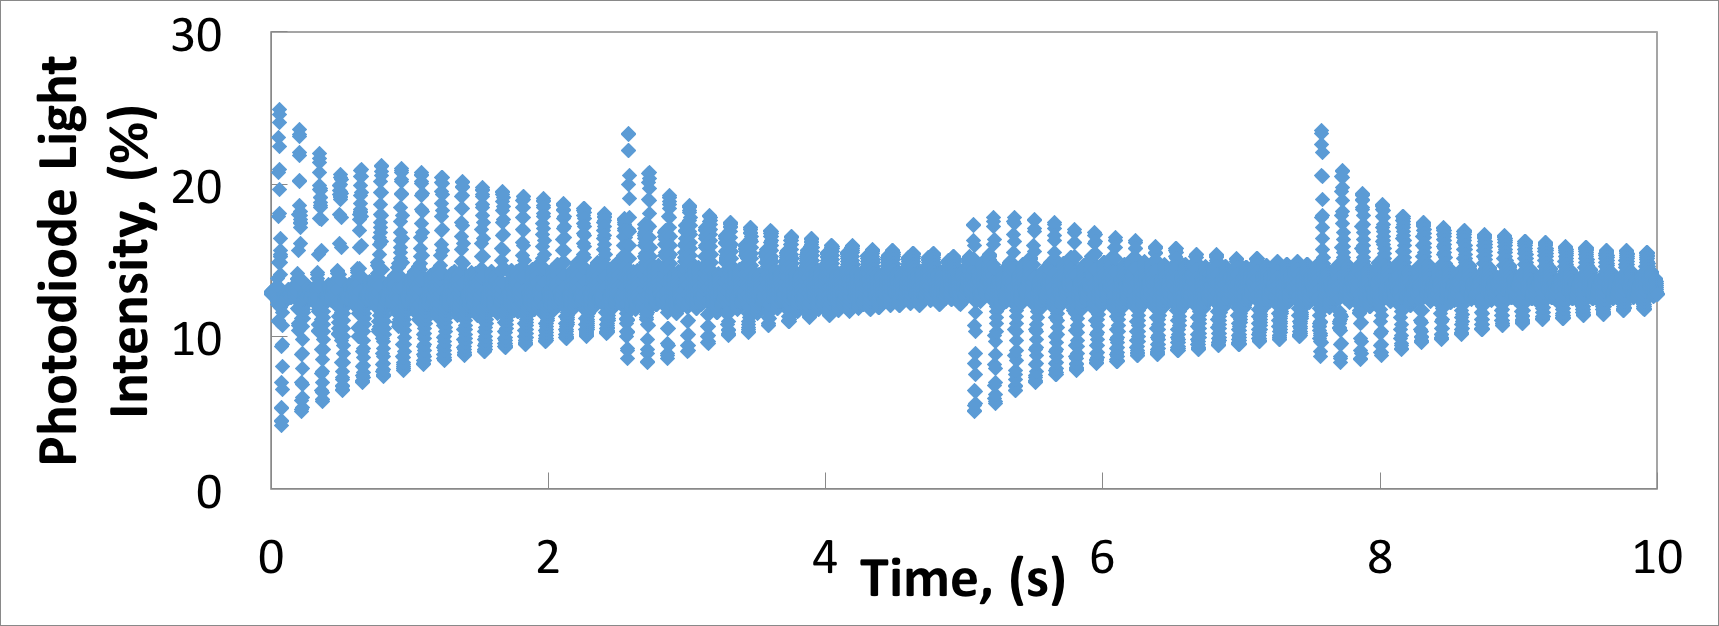
\includegraphics[width=0.95\linewidth]{LightIntensity2.png}
        \caption{Weight: 0.3 kg}
    \end{subfigure}
    \begin{subfigure}{\textwidth}
        \centering
        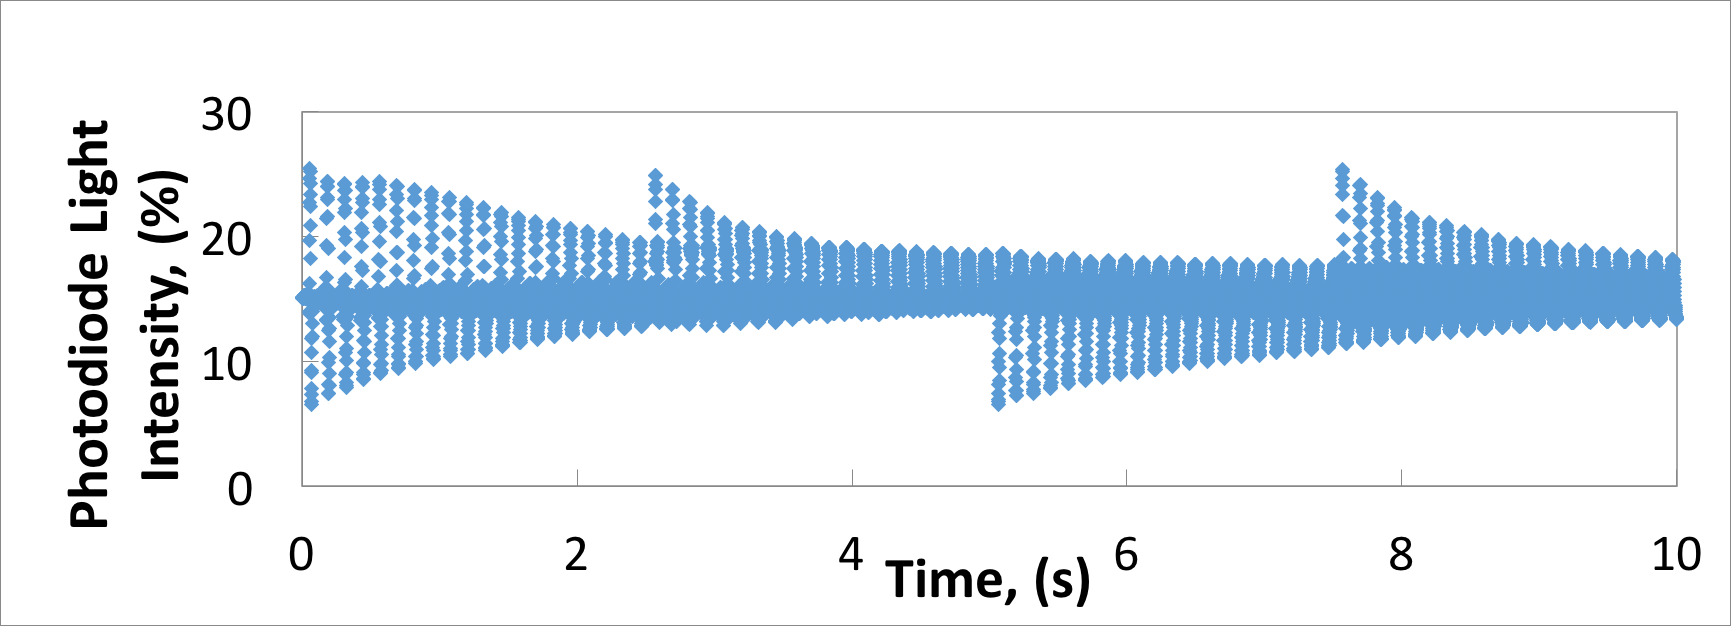
\includegraphics[width=\linewidth]{LightIntensity3.png}
        \caption{Weight: 0.4 kg}
    \end{subfigure}
    \captionsetup{labelformat=empty}
    \caption{\textbf{Figure 6.8 }
        Parametric plots of Angle (rad) vs Output voltage (V). (a) shows drive
    frequency below resonance, (b) shows drive frequency above resonance, and (c)
shows drive frequency at resonance.}
\end{figure}

A vibrating spring will produce the greatest oscillations at the fundamental
frequency, where there is one big wave traversing the string and 2 nodes of no
movement on either end of the string.  The wave produced is called an anti-node.
Higher frequencies that are a multiple of the fundamental frequencies produce
more nodes and anti-nodes.  We will try to find the frequencies that produces
these nodes in the following analysis.

To identify the fundamental frequency, we used a Lissajous plot to tune the
drive frequency until we found the Lissajous plot was as symmetric as could be.
This plot is displayed in \textbf{Figure 6.9}.  The fundamental frequency was
found to be 7.92 $\pm$ 0.01 Hz.

\begin{figure}
    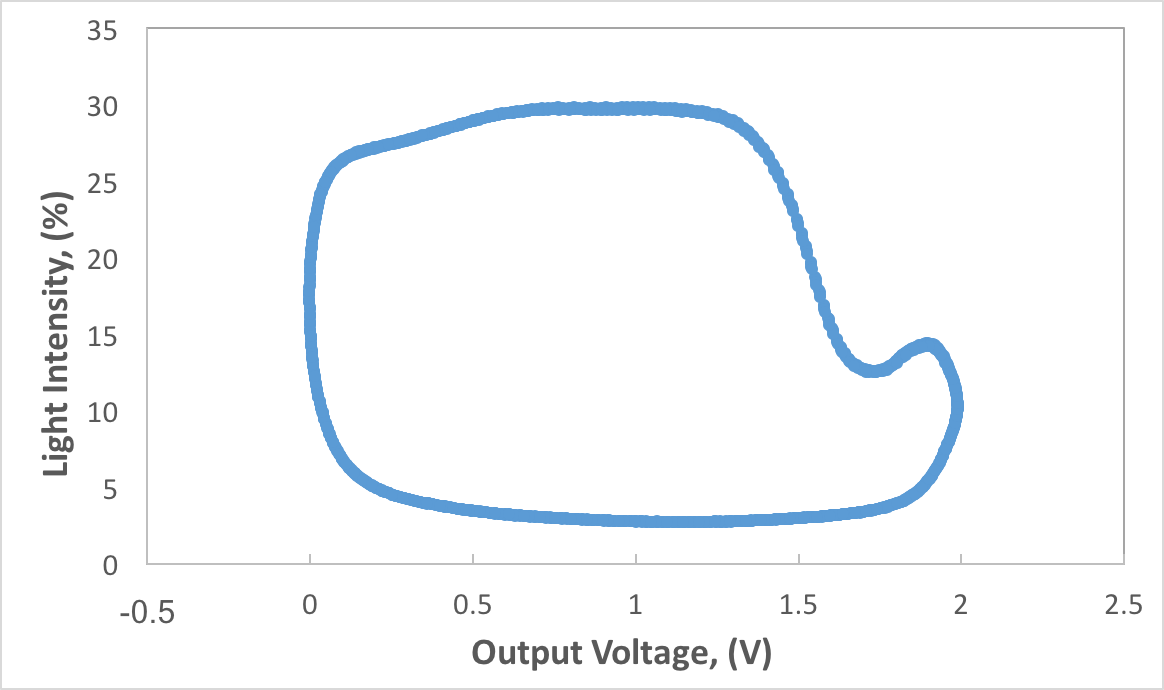
\includegraphics[width=\linewidth]{DriveFrequency.png}
    \captionsetup{labelformat=empty}
    \caption{\textbf{Figure 6.9 Light Intensity vs Voltage of Drive Frequency.}
    The parametric plot was recorded at a drive frequency of 7.92 Hz.}
\end{figure}

Now that we have the fundamental frequency, the nth normal nodes should be close
to or is a multiple of the fundamental frequency.  
The expression of the frequency of the nth normal mode is \[f(n) =
\frac{nv}{2L}\] where $n$ is the number of anti-nodes, $v$ is the wave speed,
and $L$ is the length of the string. Using the velocity measured prior for the
0.4 kg weight and the
length of the string, we approximated what the frequency should be and plotted
Lissajous plots until we found a frequency that made the plot as symmetric as it
could be.  \textbf{Table 6.3} compares the calculated to measured values of the
nth mode frequency.

\begin{center}
    \begin{tabular}{| c | c | c |}
        \hline
        Harmonic Number (n) & Measured Frequency (Hz) & Calculated Frequency (Hz) \\
        \hline
        1 & 7.92 $\pm$ 0.01 & 7.92 $\pm$ 0.01\\
        \hline
        3 & 23.81 $\pm$ 0.01 & 23.76 $\pm$ 0.04\\
        \hline
        5 & 40.02 $\pm$ 0.01 & 39.60 $\pm$ 0.07\\
        \hline
        7 & 55.78 $\pm$ 0.01 & 55.44 $\pm$ 0.09 \\
        \hline
        9 &  71.44 $\pm$ 0.01 & 71.3 $\pm$ 0.1 \\
        \hline
    \end{tabular}
\end{center}
\captionof*{table}{\textbf{Table 6.3} Measured and Calculated Harmonic
Frequencies.}

\setlength{\parindent}{5ex}
The measured frequencies were slightly higher than the predicted calculated
frequencies, yet all the measured values were within the uncertainty values of
the caluclated values, so our measurements are precise.

When a string is vibrating at a normal mode, there is no displacement at each
node.  Thus, if an object was placed on a node, it will should not interfere
with the oscillation of the standing waves. We tested this by placing a clamp 
on in the middle of the string and vibrating the string at the frequencies that
corresponded to $n=2, 4,$ and $5$, and compared the amplitudes with and without the
clamp.  \textbf{Table 6.4} shows these amplitudes.

\begin{center}
    \begin{tabular}{| c | c | c | c |}
        \hline
        Harmonic Number (n) & Drive Frequency (Hz) & Signal Amplitude Unbounded
                            & Signal Amplitude Bounded \\
        \hline
        2 & 15.84 $\pm$ 0.01 & 26.85 $\pm$ 0.01 & 26.7 $\pm$ 0.1\\
        \hline
        4 & 31.68 $\pm$ 0.01 & 23.14 $\pm$ 0.01 & 22.9 $\pm$ 0.1  \\
        \hline
        5 & 40.02 $\pm$ 0.01 & 23.32 $\pm$ 0.01 & 0.3 $\pm$ 0.1 \\
        \hline
    \end{tabular}
\end{center}
\captionof*{table}{\textbf{Table 6.4} Drive Frequency Ampltidues for bounded and
unbounded string vibrations.}

For the frequencies at $n=2$ and $n=4$, when bounded the amplitudes of
oscillation decreased, but were still within the bounds of uncertainty.  This is
to be expected, as placing a boundary condition on a node should not affect the
standing waves.  However, at $n=5$, there is almost no oscillation amplitude,
because the boundary condition is placed right on top of a node, which almost
cancels out the oscillations.

\section*{Conclusion}
\addcontentsline{toc}{section}{Conclusion}

The objective of this experiment was to study harmonic motion in two forms, the
oscillations of a physical pendulum and the waves of a vibrating string.  We
first investigated the three regimes of damping, and found that when the magnets
were spaced 15 $\pm$ 0.5 mm apart, we achieved critical damping, which is the point where
the pendulum comes to rest at the equilibrium state fastest.  

Using the same physical pendulum, we studied driven oscillations to measure the
driving resonant frequency, which was determined to be 0.714 $\pm$ 0.005 Hz.  We
also found the Q-factor of our driven harmonic oscillation, by first measuring
the damping time of the system

Potential Errors in experiment

Wave Velocities...

Wave Nodes...

Potential Errors in string experiment.


\section*{References}
\addcontentsline{toc}{section}{References}
\begin{enumerate}
    \item Campbell, W. C. et al. Physics 4AL: Mechanics Lab Manual (ver. April
        3, 2017). (Univ. California Los Angeles, Los Angeles, California).
\end{enumerate}




\end{document}



%-------------------------------------------------------------------------------
% REFERENCES
%-------------------------------------------------------------------------------
% \newpage
% \section*{References}
% \addcontentsline{toc}{section}{References}

% Anand, U., 2010. The Elusive Free Radicals, \textit{The Clinical Chemist,} [e-journal] Available at:<\url{http://www.clinchem.org/content/56/10/1649.full.pdf}> [Accessed 2 November 2013]
% \newline
% \newline

% Biology Forums, 2012. \textit{Normal glomerulus. Acute glomerulonephritis.} [online] Available at: <\url{http://biology-forums.com/index.php?action=gallery;sa=view;id=9284}> [Accessed 23 October 2013].
% \newline
% \newline

% Budisavljevic, M., Hodge, L., Barber, K., Fulmer, J., Durazo-Arvizu, R., Self, S., Kuhlmann, M., Raymond, J. and Greene, E., 2003. Oxidative stress in the pathogenesis of experimental mesangial proliferative glomerulonephritis, \textit{American Journal of Physiology - Renal Physiology,} 285(6), pp. 1138-1148.
% \newline
% \newline

% Chien, C., Lee, P., Chen, C., Ma, M., Lai, M. and Hsu, S., 2001. De Novo Demonstration and Co-localization of Free-Radical Production and Apoptosis Formation in Rat Kidney Subjected to Ischemia/Reperfusion, \textit{Journal of the American Society of Nephrology,} 12(5), pp. 973-982.
% \newline
% \newline

% Couser, W., 1993. Pathogenesis of glomerulonephritis, \textit{Kidney International Supplements,} 42, pp. 19-26.
% \newline
% \newline

% De Gasparo, M., 2002. Angiotensin II and nitric oxide interaction, \textit{Heart Failure Reviews,} [e-journal] Available at:<\url{http://www.ncbi.nlm.nih.gov/pubmed/12379820}> [Accessed 26 October 2013]
% \newline
% \newline

% Edinburgh Renal Education Pages, 2012. \textit{Glomerulonephritis} [online] Available at: <\url{http://www.edrep.org/pages/textbook/glomerulonephritis.php}> [Accessed 25 October 2013].
% \newline
% \newline

% Forbes, J., Coughlan, M. and Cooper, M., 2008. Oxidative Stress as a Major Culprit in Kidney Disease in Diabetes, \textit{Diabetes,} 57(6), pp. 1446-1454.
% \newline
% \newline

% Geeky Medics, 2010. \textit{Glomerulonephritis} [online] Available at: <\url{http://geekymedics.com/2010/10/27/glomerulonephritis/}> [Accessed 25 October 2013].
% \newline
% \newline

% Gryglewski, R., Palmer, R., Moncada, S., 1986. Superoxide anion is involved in the break­down of endothelium derived relaxing factor, \textit{Nature,} 320, pp. 454-456.
% \newline
% \newline

% Halliwell, B., 2001. Free Radicals and other reactive species in Disease, \textit{Encyclopedia of Life Sciences,} [e-journal] Available at:<\url{http://web.sls.hw.ac.uk/teaching/level4/bcm1_2/reading/oxidative_stress/files/Oxidative_stress.pdf}> [Accessed 19 October 2013]
% \newline
% \newline

% Huang, H., Patel, P. and Salahudeen, A., 2001. Lazaroid compounds prevent early but not late stages of oxidant-induced cell injury: potential explanation for the lack of efficacy of lazaroids in clinical trials, \textit{Pharmacological Research,} 41(1), pp. 55-61.
% \newline
% \newline

% Klinger, J., Abman, S. and Gladwin, M., 2013. Nitric Oxide Deficiency and Endothelial Dysfunction in Pulmonary Arterial Hypertension, \textit{American Journal of Respiratory and Critical Care Medicine,} 188(6), pp. 639-646.
% \newline
% \newline

% Lindemann, I., Boettcher, J., Oertel, K., Pasternack, R., Heine, A. and Klebe, G. 2012. Inhibitors of Transglutaminase 2: A therapeutic option in celiac disease, \textit{To be Published,} [e-journal + PDB structure] Available at:<\url{http://www.ebi.ac.uk/pdbe-srv/view/entry/3s3s/summary}> [Accessed 24 October 2013]
% \newline
% \newline

% Mayo Clinic, 2011. \textit{Glomerulonephritis} [online] Available at: <\url{http://www.mayoclinic.com/health/glomerulonephritis/DS00503/}> [Accessed 20 October 2013].
% \newline
% \newline

% McCord, J., Roy, R. and Schaffer, S., 1985. Free radicals and myocardial ischemia. The role of xanthine oxidase, \textit{Advances in myocardiology,} [e-journal] Available at:<\url{http://www.ncbi.nlm.nih.gov/pubmed/2982206}> [Accessed 24 October 2013]
% \newline
% \newline

% National Health Service, 2012. \textit{Causes of glomerulonephritis} [online] Available at: <\url{http://www.nhs.uk/Conditions/Glomerulonephritis/Pages/Causes.aspx}> [Accessed 20 October 2013].
% \newline
% \newline

% Niaudet, P., 2013. \textit{Overview of the pathogenesis and causes of glomerulonephritis in children.} [online] Available at: <\url{http://www.uptodate.com/contents/overview-of- \ the-pathogenesis-and-causes-of-glomerulonephritis-in-children}> [Accessed 21 October 2013].
% \newline
% \newline

% Ronco, P., 2013. \textit{Mechanisms of glomerular crescent formation.} [online] Available at: <\url{http://www.uptodate.com/contents/mechanisms-of-glomerular-crescent-formation}> [Accessed 21 October 2013].
% \newline
% \newline

% Rutchik, J., 2013. \textit{Toxic Neuropathy Clinical Presentation.} [online] Available at: <\url{http://emedicine.medscape.com/article/1175276-clinical#a0216}> [Accessed 26 October 2013].
% \newline
% \newline

% R\&D Systems, 2013. \textit{Technical Information. Ischemia/Reperfusion Injury.} [online] Available at: <\url{http://www.rndsystems.com/cb_detail_objectname_SP96_Ischemia.aspx}> [Accessed 28 October 2013].
% \newline
% \newline

% Salahudeen, A., 1999. Free Radicals in Kidney Disease and Transplantation, \textit{Saudi Journal of Kidney Diseases and Transplantation,} 10(2), pp. 137-143.
% \newline
% \newline

% Sarma, A., Mallick, A. and Ghosh, A., 2010. Free Radicals and Their Role in Different Clinical Conditions: An Overview, \textit{International Journal of Pharma Sciences and Research,} 1(3), pp. 182-192.
% \newline
% \newline

% Shah, S., Baliga, R., Rajapurkar, M. and Fonseca, V., 2007. Oxidants in Chronic Kidney Disease, \textit{Journal of the American Society of Nephrology,} 18(1), pp. 16-28.
% \newline
% \newline

% The University of Utah, Unknown. \textit{Glomerulonephritis} [online] Available at: <\url{http://library.med.utah.edu/WebPath/RENAHTML/RENALIDX.html#8}> [Accessed 25 October 2013].
% \newline
% \newline

% Wang, C. and Salahudeen, A., 1994. Cyclosporine nephrotoxicity: attenuation by an antioxidant -inhibitor of lipid peroxidation in-vitro and in-vivo, \textit{Transplantation,} 58, pp. 940-946.
% \newline
% \newline

% Wang, C. and Salahudeen, A., 1995. Lipid peroxidation accompanies cyclosporine nephrotoxicity: effects of vitamin E, \textit{Kidney International,} 47, pp. 927-934.
% \newline
% \newline

% Weiss, S., 1989. Tissue Destruction by Neutrophils, \textit{New England Journal of Medicine,} 320, pp. 365-376.
% \newline
% \newline



%-------------------------------------------------------------------------------
% SNIPPETS
%-------------------------------------------------------------------------------

%\begin{figure}[!ht]
%    \centering
%    \includegraphics[width=0.8\textwidth]{file_name}
%    \caption{}
%    \centering
%    \label{label:file_name}
%\end{figure}

%\begin{figure}[!ht]
%    \centering
%    \includegraphics[width=0.8\textwidth]{graph}
%    \caption{Blood pressure ranges and associated level of hypertension (American Heart Association, 2013).}
%    \centering
%    \label{label:graph}
%\end{figure}

%\begin{wrapfigure}{r}{0.30\textwidth}
%    \vspace{-40pt}
%    \begin{center}
%        \includegraphics[width=0.29\textwidth]{file_name}
%    \end{center}
%    \vspace{-20pt}
%    \caption{}
%    \label{label:file_name}
%\end{wrapfigure}

%\begin{wrapfigure}{r}{0.45\textwidth}
%    \begin{center}
%        \includegraphics[width=0.29\textwidth]{manometer}
%    \end{center}
%    \caption{Aneroid sphygmomanometer with stethoscope (Medicalexpo, 2012).}
%    \label{label:manometer}
%\end{wrapfigure}

%\begin{table}[!ht]\footnotesize
%    \centering
%    \begin{tabular}{cccccc}
%    \toprule
%    \multicolumn{2}{c} {Pearson's correlation test} & \multicolumn{4}{c} {Independent t-test} \\
%    \midrule    
%    \multicolumn{2}{c} {Gender} & \multicolumn{2}{c} {Activity level} & \multicolumn{2}{c} {Gender} \\
%    \midrule
%    Males & Females & 1st level & 6th level & Males & Females \\
%    \midrule
%    \multicolumn{2}{c} {BMI vs. SP} & \multicolumn{2}{c} {Systolic pressure} & \multicolumn{2}{c} {Systolic Pressure} \\
%    \multicolumn{2}{c} {BMI vs. DP} & \multicolumn{2}{c} {Diastolic pressure} & \multicolumn{2}{c} {Diastolic pressure} \\
%    \multicolumn{2}{c} {BMI vs. MAP} & \multicolumn{2}{c} {MAP} & \multicolumn{2}{c} {MAP} \\
%    \multicolumn{2}{c} {W:H ratio vs. SP} & \multicolumn{2}{c} {BMI} & \multicolumn{2}{c} {BMI} \\
%    \multicolumn{2}{c} {W:H ratio vs. DP} & \multicolumn{2}{c} {W:H ratio} & \multicolumn{2}{c} {W:H ratio} \\
%    \multicolumn{2}{c} {W:H ratio vs. MAP} & \multicolumn{2}{c} {\% Body fat} & \multicolumn{2}{c} {\% Body fat} \\
%    \multicolumn{2}{c} {} & \multicolumn{2}{c} {Height} & \multicolumn{2}{c} {Height} \\
%    \multicolumn{2}{c} {} & \multicolumn{2}{c} {Weight} & \multicolumn{2}{c} {Weight} \\
%    \multicolumn{2}{c} {} & \multicolumn{2}{c} {Heart rate} & \multicolumn{2}{c} {Heart rate} \\
%    \bottomrule
%    \end{tabular}
%    \caption{Parameters that were analysed and related statistical test performed for current study. BMI - body mass index; SP - systolic pressure; DP - diastolic pressure; MAP - mean arterial pressure; W:H ratio - waist to hip ratio.}
%    \label{label:tests}
%\end{table}
